\documentclass[12pt, twoside]{article}
\usepackage[letterpaper, margin=1in, headsep=0.5in]{geometry}
\usepackage[english]{babel}
\usepackage[utf8]{inputenc}
\usepackage{amsmath}
\usepackage{amsfonts}
\usepackage{amssymb}
\usepackage{tikz}
\usetikzlibrary{quotes, angles}
\usepackage{graphicx}
\usepackage{enumitem}
\usepackage{multicol}

\newif\ifmeta
\metatrue %print standards and topics tags

\title{Regents Geometry}
\author{Chris Huson}
\date{December 2021}

\usepackage{fancyhdr}
\pagestyle{fancy}
\fancyhf{}
\renewcommand{\headrulewidth}{0pt} % disable the underline of the header
\raggedbottom


\fancyhead[LE]{\thepage}
\fancyhead[RO]{\thepage \\ Name: \hspace{4cm} \,\\}
\fancyhead[LO]{BECA / Dr. Huson / Geometry 5 Congruence Transformations}

\begin{document}

\subsubsection*{5.5 Classwork: Mixed congruence transformations \hfill CCSS.HSG.CO.A.5}
\begin{enumerate}
\item Plot the parallelogram $BECA$ with $B(-2,-1)$, $E(3,-1)$, $C(2,-4)$, and $A(-3,-4)$. Translate the quadrilateral up 5 and right 2, labeling it $B'E'C'A'$. (use a straight edge for full credit)
    \begin{center}
      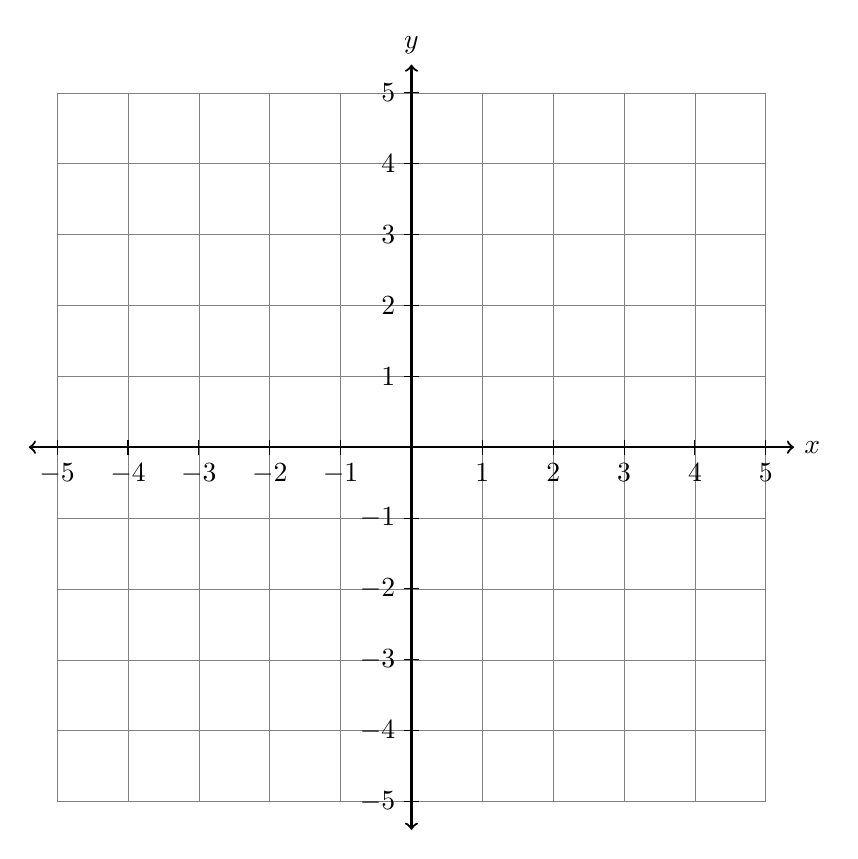
\begin{tikzpicture}[scale=0.9]
      \draw [help lines] (-5,-5) grid (5,5);
      \draw [thick, <->] (-5.4,0) -- (5.4,0) node [right] {$x$};
      \draw [thick, <->] (0,-5.4)--(0,5.4) node [above] {$y$};
      \foreach \x in {-5,...,-1,1,2,3,4,5}
        \draw[shift={(\x,0)},color=black] (0pt,-3pt) -- (0pt,3pt) node[below=5pt]  {$\x$};
      \foreach \y in {-5,...,-1,1,2,3,4,5}
        \draw[shift={(0,\y)},color=black] (-3pt,0pt) -- (3pt,0pt) node[left=5pt]  {$\y$}; 
    \end{tikzpicture}
  \end{center}
  
  \item Reflect the triangle over the $x$-axis, $\triangle ABC \rightarrow \triangle A'B'C'$. Complete the table of the coordinates and plot and label the image on the grid. \vspace{0.5cm}
  \begin{multicols}{2}
    $A(1,2) \rightarrow$ \\[0.7cm]
    $B(1,4) \rightarrow$ \\[0.7cm]
    $C(4,2) \rightarrow$ \\[0.7cm]
      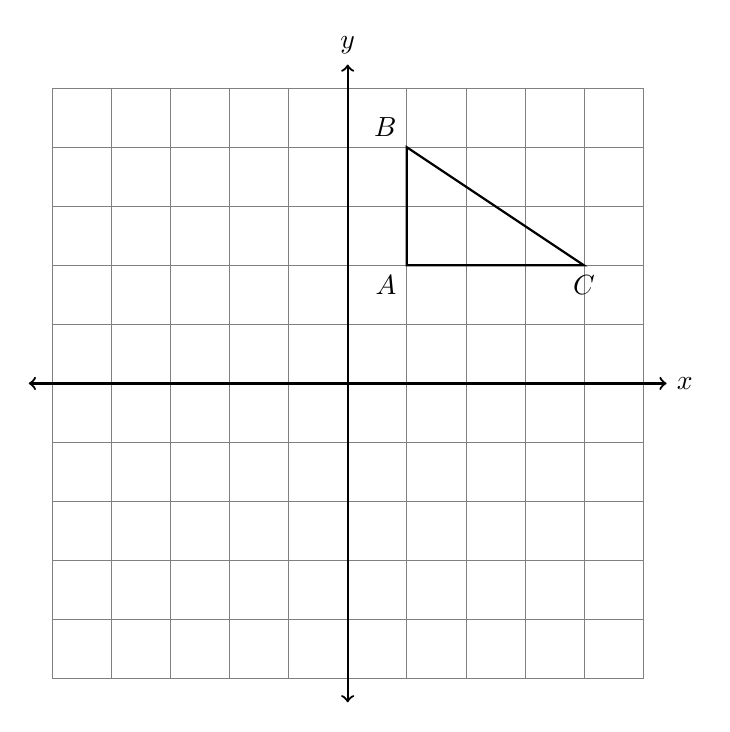
\begin{tikzpicture}[scale=.75]
      \draw [help lines] (-5,-5) grid (5,5);
      \draw [thick, <->] (-5.4,0) -- (5.4,0) node [right] {$x$};
      \draw [thick, <->] (0,-5.4)--(0,5.4) node [above] {$y$};  
      \draw [thick]
        (1,2) node[below left] {$A$}--
        (1,4) node[above left] {$B$}--
        (4,2) node[below] {$C$}--cycle;  
      \end{tikzpicture}
    \end{multicols}

\newpage
\item A translation is performed mapping $(x,y) \rightarrow (x+4, y-1)$.
\begin{multicols}{2}
  \begin{enumerate}
    \item What is the horizontal shift, how many squares right or left? \vspace{1cm}
    \item What is the vertical shift, how many squares up or down? \vspace{1cm}
    \item Identify the image of point $A$. $A(-1,2)\rightarrow$
  \end{enumerate}
    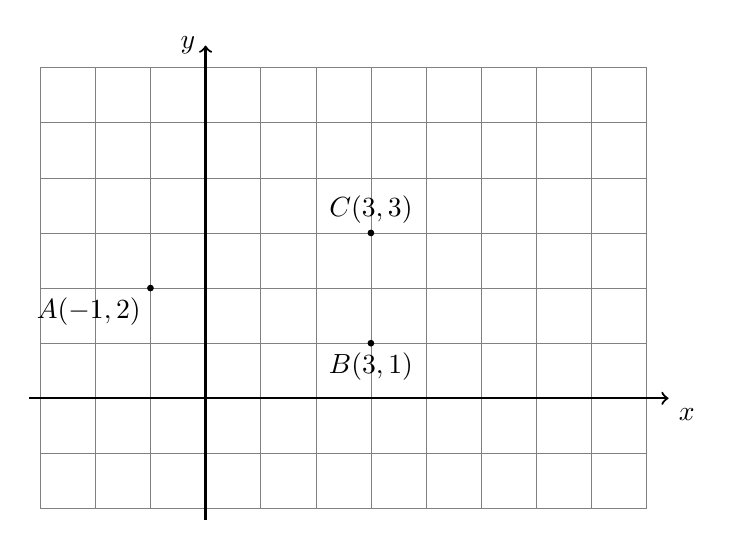
\begin{tikzpicture}[scale=0.7]
      \draw [help lines] (-3,-2) grid (8,6);
      \draw [thick, ->] (-3.2,0) -- (8.4,0) node [below right] {$x$};
      \draw [thick, ->] (0,-2.2)--(0,6.4) node [left] {$y$};
      \draw [fill] (3,1) circle [radius=0.05] node[below] {$B(3,1)$};
      \draw [fill] (-1,2) circle [radius=0.05] node[below left] {$A(-1,2)$};
      %\draw [->, dashed] (7,1)--(2,3);
      \draw [fill] (3,3) circle [radius=0.05] node[above] {$C(3,3)$};
    \end{tikzpicture}
  \end{multicols} \vspace{1cm}

\item In the diagram below, $\triangle ABC$ with sides of 13, 15, and 16, is mapped onto $\triangle DEF$ after a clockwise rotation of $90^\circ$ about point $P$. 
  \begin{multicols}{2}
    \begin{enumerate}
      \item What is $A$ mapped to? $A \rightarrow$ \vspace{1.5cm}
      \item What corresponds to $F$? \vspace{1.5cm}
      \item Given $DE=2x-1$. Find $x$. \vspace{1.5cm}
    \end{enumerate}
    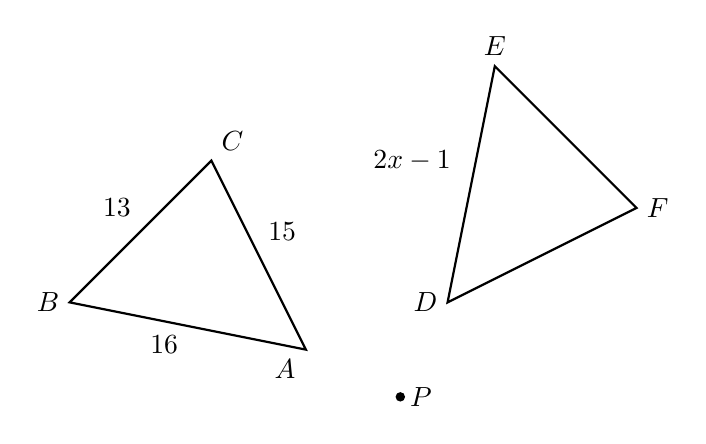
\begin{tikzpicture}[scale=.6]
      %\draw [thick, <->] (-7.4,0) -- (10.4,0) node [right] {$x$};
      %draw [thick, <->] (0,-5.4)--(0,10.4) node [above] {$y$};
      \fill (0,0) circle[radius=0.1] node[right]{$P$};
      \draw [thick]
        (-2,1) node[below left] {$A$}--
        (-7,2) node[left] {$B$}--
        (-4,5) node[above right] {$C$}--cycle;
        \node at (-5,1.5)[below]{16};
        \node at (-6,4){13};
        \node at (-2.5,3.5){15};
        \node at (0.25,5){$2x-1$};
      \draw [thick]
        (1,2) node[left] {$D$}--
        (2,7) node[above] {$E$}--
        (5,4) node[right] {$F$}--cycle;
    \end{tikzpicture}
  \end{multicols}
  \vspace{3cm}

\item A translation maps $D(2,4) \rightarrow D'(-3,4)$. What is the image of $E(5,-5)$ under the same translation?

\newpage
\item The triangle $ABC$, shown below, undergoes two rigid motions carrying it onto triangle $XYZ$. State the two isometric transformations. (be specific)
  \begin{flushright}
    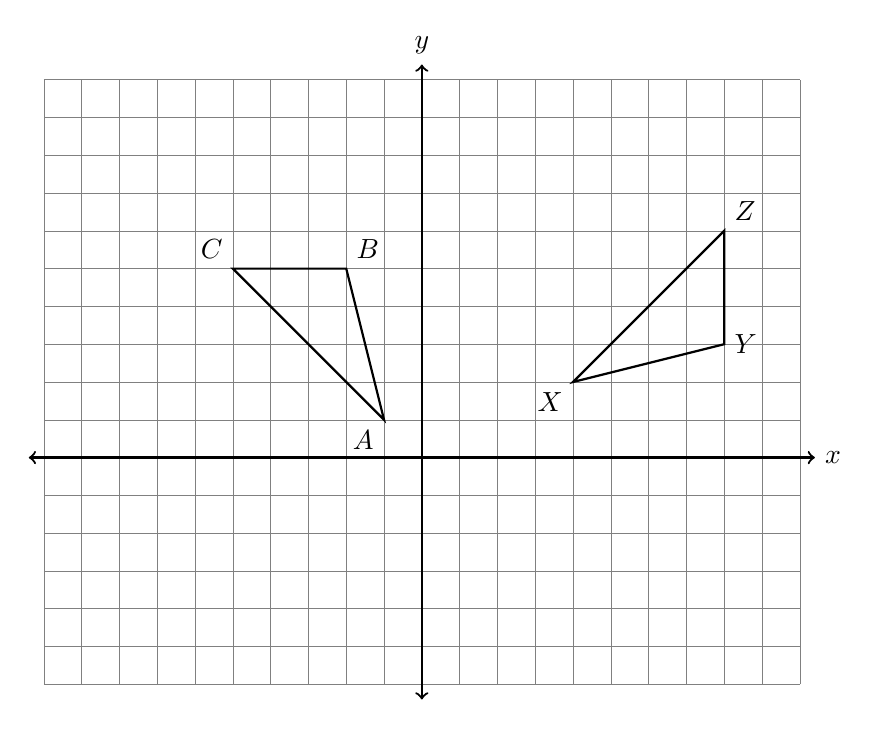
\begin{tikzpicture}[scale=.48]
      \draw [help lines] (-10,-6) grid (10,10);
      \draw [thick, <->] (-10.4,0) -- (10.4,0) node [right] {$x$};
      \draw [thick, <->] (0,-6.4)--(0,10.4) node [above] {$y$};
      \draw [thick]
        (4,2) node[below left] {$X$}--
        (8,3) node[right] {$Y$}--
        (8,6) node[above right] {$Z$}--cycle;
      \draw [thick]
        (-1,1) node[below left] {$A$}--
        (-2,5) node[above right] {$B$}--
        (-5,5) node[above left] {$C$}--cycle;
    \end{tikzpicture}
  \end{flushright}

\item Triangle $\triangle ABC$ is graphed on the set of axes below. The vertices of $\triangle ABC$ have the coordinates $A(2,-3)$, $B(8,1)$, and $C(-1,8)$. \\*[0.25cm]
Reflect the triangle across the $y$-axis. Write down its coordinates in a table and plot and label it on the graph.
    \begin{flushright} %4 quadrant regents grid
    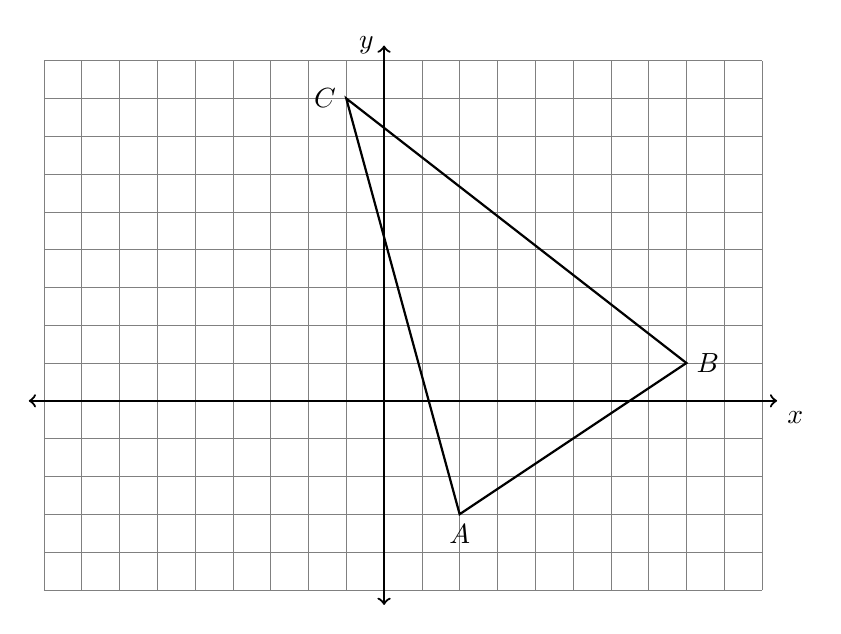
\begin{tikzpicture}[scale=.48]
      \draw [help lines] (-9,-5) grid (10,9);
      \draw [thick, <->] (-9.4,0) -- (10.4,0) node [below right] {$x$};
      \draw [thick, <->] (0,-5.4)--(0,9.4) node [left] {$y$};
      \draw [thick] (2,-3) node[below] {$A$}--
      (8,1) node[right] {$B$}--
      (-1,8) node[left] {$C$}--
      cycle;
      %\draw [fill] (5,0) circle [radius=0.1] node[above left] {$P$};
    \end{tikzpicture}
    \end{flushright}

\newpage
\item In  $\triangle ABC$ shown below, side $\overline{AC}$ is extended to point $D$ with $m\angle DAB=(6x-16)^\circ$, $m\angle C=(x+4)^\circ$, and $m\angle B=(4x+3)^\circ$. \\[0.25cm]
Find $m\angle BAC$.
\begin{flushright}
    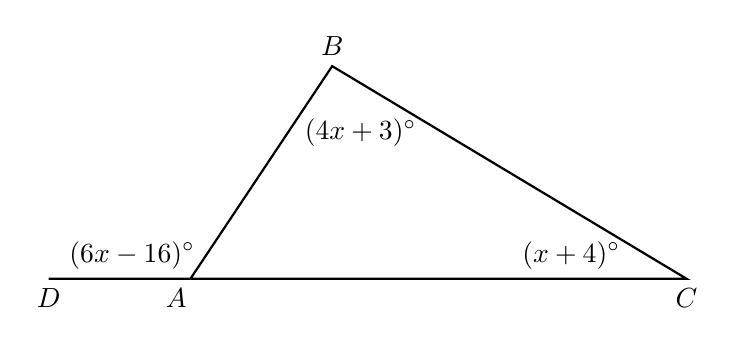
\begin{tikzpicture}[scale=0.9]
      \draw [thick](0,0)node[below]{$D$}--
        (1.8,0)node[below]{$A$}--
        (9,0)node[below]{$C$}--
        (4,3)node[above]{$B$} --(2,0);
        \node at (2.2,0)[above left]{$(6x-16)^\circ$};
        \node at (8.2,0)[above left]{$(x+4)^\circ$};
        \node at (4.4,2.4)[below]{$(4x+3)^\circ$};
    \end{tikzpicture}
  \end{flushright} \vspace{1cm}

  \item The quadrilateral $ROCK$ undergoes rigid motions, shown below. Describe the sequence of transformations applied.
  \begin{flushright}
      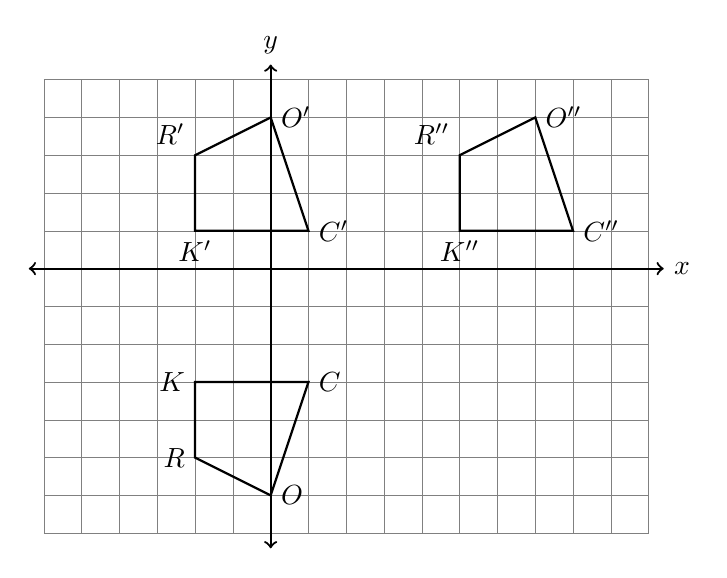
\begin{tikzpicture}[scale=.48]
      \draw [help lines] (-6,-7) grid (10,5);
      \draw [thick, <->] (-6.4,0) -- (10.4,0) node [right] {$x$};
      \draw [thick, <->] (0,-7.4)--(0,5.4) node [above] {$y$};  
      \draw [thick]
        (5,1) node[below] {$K''$}--
        (5,3) node[above left] {$R''$}--
        (7,4) node[right] {$O''$}--
        (8,1) node[right] {$C''$}--cycle;
      \draw [thick]
        (-2,1) node[below] {$K'$}--
        (-2,3) node[above left] {$R'$}--
        (0,4) node[right] {$O'$}--
        (1,1) node[right] {$C'$}--cycle;  
      \draw [thick]
      (-2,-3) node[left] {$K$}--
      (-2,-5) node[left] {$R$}--
      (0,-6) node[right] {$O$}--
      (1,-3) node[right] {$C$}--cycle;
    \end{tikzpicture}
  \end{flushright}

  \item The quadrilateral $MATH$ is mapped to $M'A'T'H'$ by a rigid motion. What transformation a been applied?
  \begin{multicols}{2}
    \begin{enumerate}
      \item Dilation
      \item Reflection
      \item Rotation
      \item Translation
    \end{enumerate}
    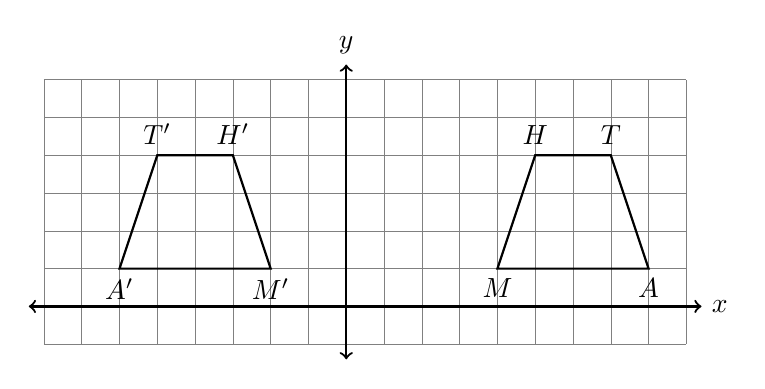
\begin{tikzpicture}[scale=.48]
      \draw [help lines] (-8,-1) grid (9,6);
      \draw [thick, <->] (-8.4,0) -- (9.4,0) node [right] {$x$};
      \draw [thick, <->] (0,-1.4)--(0,6.4) node [above] {$y$};  
      \draw [thick]
        (4,1) node[below] {$M$}--
        (8,1) node[below] {$A$}--
        (7,4) node[above] {$T$}--
        (5,4) node[above] {$H$}--cycle;
      \draw [thick]
        (-2,1) node[below] {$M'$}--
        (-6,1) node[below] {$A'$}--
        (-5,4) node[above] {$T'$}--
        (-3,4) node[above] {$H'$}--cycle; 
    \end{tikzpicture}
  \end{multicols}

\end{enumerate}
\end{document}